\documentclass{standalone}
\usepackage{tikz}
\usetikzlibrary{patterns, positioning}
\usepackage[sfdefault]{ClearSans} %% option 'sfdefault' activates Clear Sans as the default text font
\usepackage[T1]{fontenc}

\begin{document}
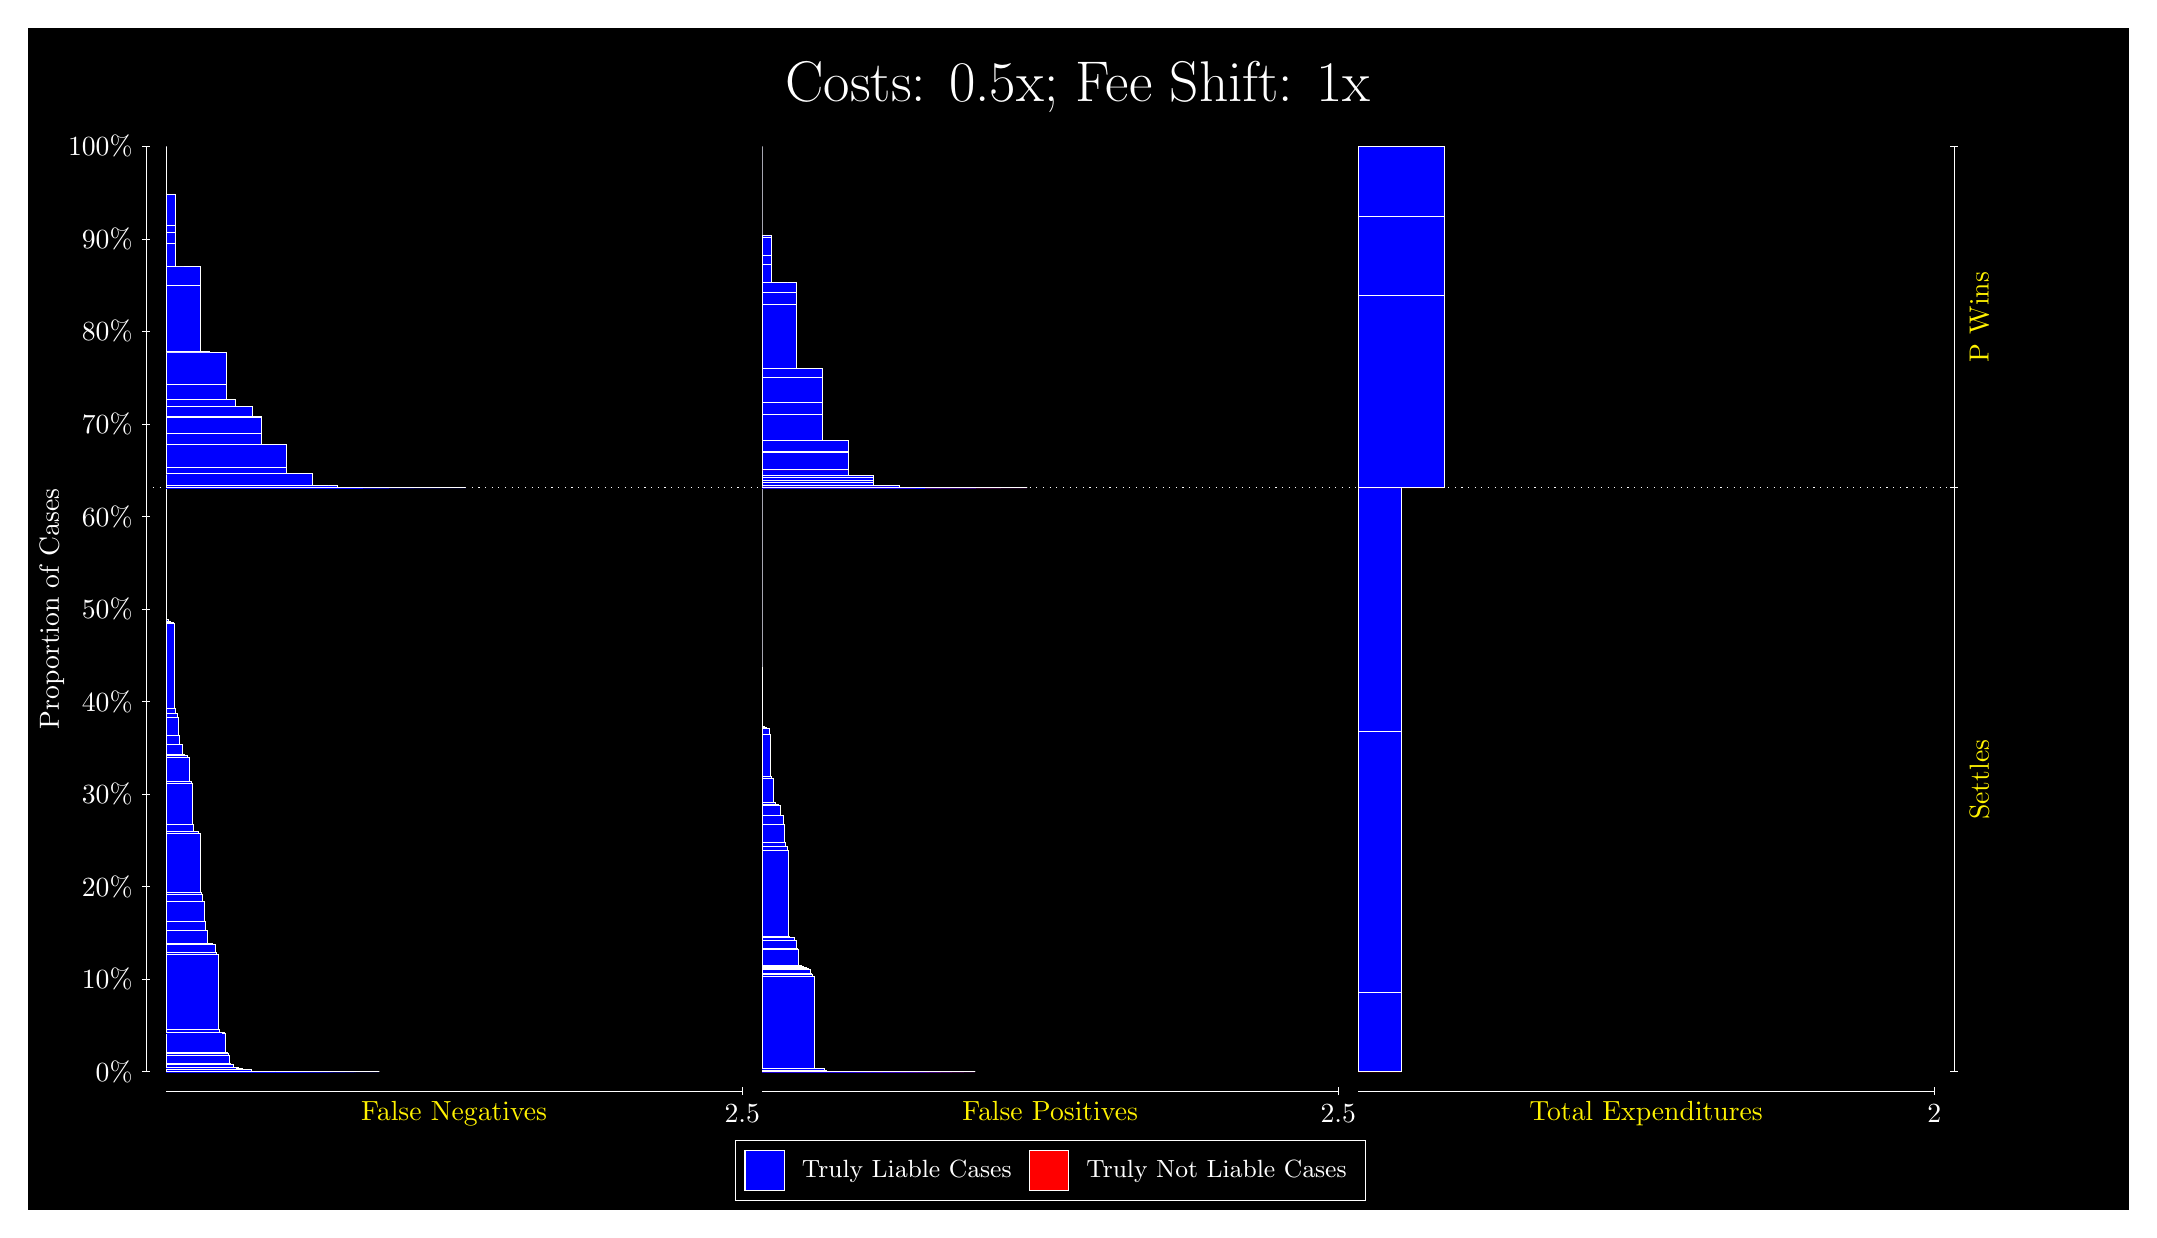
\begin{tikzpicture}
\draw[fill=black] (0,0) rectangle (26.667,15);
\draw[text=white] (0,13.5) rectangle (26.667,15) node[midway] {\huge Costs: 0.5x; Fee Shift: 1x};
\draw[white, very thin] (1.5,1.75) -- (1.5,13.5);
\node[rotate=90, text=white, anchor=center] at (0.3, 7.625) {Proportion of Cases};
\draw[white, very thin] (1.45,1.75) -- (1.55,1.75);
\node[text=white, anchor=east] at (1.45, 1.75) {0\%};
\draw[white, very thin] (1.45,2.925) -- (1.55,2.925);
\node[text=white, anchor=east] at (1.45, 2.925) {10\%};
\draw[white, very thin] (1.45,4.1) -- (1.55,4.1);
\node[text=white, anchor=east] at (1.45, 4.1) {20\%};
\draw[white, very thin] (1.45,5.275) -- (1.55,5.275);
\node[text=white, anchor=east] at (1.45, 5.275) {30\%};
\draw[white, very thin] (1.45,6.45) -- (1.55,6.45);
\node[text=white, anchor=east] at (1.45, 6.45) {40\%};
\draw[white, very thin] (1.45,7.625) -- (1.55,7.625);
\node[text=white, anchor=east] at (1.45, 7.625) {50\%};
\draw[white, very thin] (1.45,8.8) -- (1.55,8.8);
\node[text=white, anchor=east] at (1.45, 8.8) {60\%};
\draw[white, very thin] (1.45,9.975) -- (1.55,9.975);
\node[text=white, anchor=east] at (1.45, 9.975) {70\%};
\draw[white, very thin] (1.45,11.15) -- (1.55,11.15);
\node[text=white, anchor=east] at (1.45, 11.15) {80\%};
\draw[white, very thin] (1.45,12.325) -- (1.55,12.325);
\node[text=white, anchor=east] at (1.45, 12.325) {90\%};
\draw[white, very thin] (1.45,13.5) -- (1.55,13.5);
\node[text=white, anchor=east] at (1.45, 13.5) {100\%};

\draw[white, very thin] (24.457,1.75) -- (24.457,13.5);
\draw[white, very thin] (24.407,1.75) -- (24.507,1.75);
\node[anchor=west] at (24.407, 1.75) {};
\draw[white, very thin] (24.407,9.1636) -- (24.507,9.1636);
\node[anchor=west] at (24.407, 9.1636) {};
\draw[white, very thin] (24.407,13.5) -- (24.507,13.5);
\node[anchor=west] at (24.407, 13.5) {};

\draw[white, very thin, fill=blue] (1.75,1.75) rectangle (4.458,1.75);
\draw[white, very thin, fill=blue] (1.75,1.75) rectangle (4.1652,1.75);
\draw[white, very thin, fill=blue] (1.75,1.75) rectangle (4.1327,1.75);
\draw[white, very thin, fill=blue] (1.75,1.75) rectangle (4.0188,1.75);
\draw[white, very thin, fill=blue] (1.75,1.75) rectangle (3.8725,1.75);
\draw[white, very thin, fill=blue] (1.75,1.75) rectangle (3.8399,1.75);
\draw[white, very thin, fill=blue] (1.75,1.75) rectangle (3.8074,1.75);
\draw[white, very thin, fill=blue] (1.75,1.75) rectangle (3.7261,1.75);
\draw[white, very thin, fill=blue] (1.75,1.75) rectangle (3.6936,1.75);
\draw[white, very thin, fill=blue] (1.75,1.75) rectangle (3.5797,1.75);
\draw[white, very thin, fill=blue] (1.75,1.75) rectangle (3.5472,1.75);
\draw[white, very thin, fill=blue] (1.75,1.75) rectangle (3.5147,1.75);
\draw[white, very thin, fill=blue] (1.75,1.75) rectangle (3.4821,1.75);
\draw[white, very thin, fill=blue] (1.75,1.75) rectangle (3.4333,1.75);
\draw[white, very thin, fill=blue] (1.75,1.75) rectangle (3.4008,1.75);
\draw[white, very thin, fill=blue] (1.75,1.75) rectangle (3.3683,1.75);
\draw[white, very thin, fill=blue] (1.75,1.75) rectangle (3.287,1.75);
\draw[white, very thin, fill=blue] (1.75,1.75) rectangle (3.2544,1.75);
\draw[white, very thin, fill=blue] (1.75,1.75) rectangle (3.2219,1.75);
\draw[white, very thin, fill=blue] (1.75,1.75) rectangle (3.1894,1.75);
\draw[white, very thin, fill=blue] (1.75,1.75) rectangle (3.1568,1.7505);
\draw[white, very thin, fill=blue] (1.75,1.7505) rectangle (3.1406,1.7505);
\draw[white, very thin, fill=blue] (1.75,1.7505) rectangle (3.1081,1.7505);
\draw[white, very thin, fill=blue] (1.75,1.7505) rectangle (3.0755,1.7506);
\draw[white, very thin, fill=blue] (1.75,1.7506) rectangle (3.043,1.7507);
\draw[white, very thin, fill=blue] (1.75,1.7507) rectangle (2.9942,1.7508);
\draw[white, very thin, fill=blue] (1.75,1.7508) rectangle (2.9617,1.7508);
\draw[white, very thin, fill=blue] (1.75,1.7508) rectangle (2.9292,1.7526);
\draw[white, very thin, fill=blue] (1.75,1.7526) rectangle (2.8966,1.753);
\draw[white, very thin, fill=blue] (1.75,1.753) rectangle (2.8641,1.7548);
\draw[white, very thin, fill=blue] (1.75,1.7548) rectangle (2.8478,1.7548);
\draw[white, very thin, fill=blue] (1.75,1.7548) rectangle (2.8316,1.779);
\draw[white, very thin, fill=blue] (1.75,1.779) rectangle (2.8153,1.7791);
\draw[white, very thin, fill=blue] (1.75,1.7791) rectangle (2.7828,1.7791);
\draw[white, very thin, fill=blue] (1.75,1.7791) rectangle (2.7502,1.7831);
\draw[white, very thin, fill=blue] (1.75,1.7831) rectangle (2.7177,1.7873);
\draw[white, very thin, fill=blue] (1.75,1.7873) rectangle (2.7015,1.7975);
\draw[white, very thin, fill=blue] (1.75,1.7975) rectangle (2.6689,1.7978);
\draw[white, very thin, fill=blue] (1.75,1.7978) rectangle (2.6364,1.7982);
\draw[white, very thin, fill=blue] (1.75,1.7982) rectangle (2.6039,1.8378);
\draw[white, very thin, fill=blue] (1.75,1.8378) rectangle (2.5713,1.8551);
\draw[white, very thin, fill=blue] (1.75,1.8551) rectangle (2.5551,1.9573);
\draw[white, very thin, fill=blue] (1.75,1.9573) rectangle (2.5388,1.9874);
\draw[white, very thin, fill=blue] (1.75,1.9874) rectangle (2.5225,1.9891);
\draw[white, very thin, fill=blue] (1.75,1.9891) rectangle (2.5063,2.2396);
\draw[white, very thin, fill=blue] (1.75,2.2396) rectangle (2.49,2.2424);
\draw[white, very thin, fill=blue] (1.75,2.2424) rectangle (2.4575,2.243);
\draw[white, very thin, fill=blue] (1.75,2.243) rectangle (2.425,2.2846);
\draw[white, very thin, fill=blue] (1.75,2.2846) rectangle (2.4087,3.2436);
\draw[white, very thin, fill=blue] (1.75,3.2436) rectangle (2.3924,3.2664);
\draw[white, very thin, fill=blue] (1.75,3.2664) rectangle (2.3762,3.3698);
\draw[white, very thin, fill=blue] (1.75,3.3698) rectangle (2.3436,3.3748);
\draw[white, very thin, fill=blue] (1.75,3.3748) rectangle (2.3111,3.3814);
\draw[white, very thin, fill=blue] (1.75,3.3814) rectangle (2.2786,3.5469);
\draw[white, very thin, fill=blue] (1.75,3.5469) rectangle (2.2461,3.6556);
\draw[white, very thin, fill=blue] (1.75,3.6556) rectangle (2.2298,3.9109);
\draw[white, very thin, fill=blue] (1.75,3.9109) rectangle (2.2135,3.9985);
\draw[white, very thin, fill=blue] (1.75,3.9985) rectangle (2.1973,4.0236);
\draw[white, very thin, fill=blue] (1.75,4.0236) rectangle (2.181,4.7793);
\draw[white, very thin, fill=blue] (1.75,4.7793) rectangle (2.1647,4.797);
\draw[white, very thin, fill=blue] (1.75,4.797) rectangle (2.1322,4.8002);
\draw[white, very thin, fill=blue] (1.75,4.8002) rectangle (2.0997,4.8838);
\draw[white, very thin, fill=blue] (1.75,4.8838) rectangle (2.0834,5.4103);
\draw[white, very thin, fill=blue] (1.75,5.4103) rectangle (2.0672,5.434);
\draw[white, very thin, fill=blue] (1.75,5.434) rectangle (2.0509,5.7409);
\draw[white, very thin, fill=blue] (1.75,5.7409) rectangle (2.0184,5.7635);
\draw[white, very thin, fill=blue] (1.75,5.7635) rectangle (1.9858,5.7802);
\draw[white, very thin, fill=blue] (1.75,5.7802) rectangle (1.9533,5.9118);
\draw[white, very thin, fill=blue] (1.75,5.9118) rectangle (1.9208,6.0206);
\draw[white, very thin, fill=blue] (1.75,6.0206) rectangle (1.9045,6.2473);
\draw[white, very thin, fill=blue] (1.75,6.2473) rectangle (1.8882,6.2967);
\draw[white, very thin, fill=blue] (1.75,6.2967) rectangle (1.872,6.359);
\draw[white, very thin, fill=blue] (1.75,6.359) rectangle (1.8557,7.4426);
\draw[white, very thin, fill=blue] (1.75,7.4426) rectangle (1.8395,7.4603);
\draw[white, very thin, fill=blue] (1.75,7.4603) rectangle (1.8069,7.4634);
\draw[white, very thin, fill=blue] (1.75,7.4634) rectangle (1.7744,7.4933);
\draw[white, very thin, fill=blue] (1.75,7.4933) rectangle (1.7581,7.602);
\draw[white, very thin, fill=red] (1.75,7.602) rectangle (1.75,7.602);
\draw[white, very thin, fill=blue] (1.75,7.602) rectangle (1.75,9.1636);
\draw[white, very thin, fill=blue] (1.75,9.1636) rectangle (5.5558,9.1636);
\draw[white, very thin, fill=blue] (1.75,9.1636) rectangle (5.2305,9.1636);
\draw[white, very thin, fill=blue] (1.75,9.1636) rectangle (4.9052,9.1637);
\draw[white, very thin, fill=blue] (1.75,9.1637) rectangle (4.58,9.1637);
\draw[white, very thin, fill=blue] (1.75,9.1637) rectangle (4.58,9.1639);
\draw[white, very thin, fill=blue] (1.75,9.1639) rectangle (4.4661,9.1639);
\draw[white, very thin, fill=blue] (1.75,9.1639) rectangle (4.2547,9.1657);
\draw[white, very thin, fill=blue] (1.75,9.1657) rectangle (4.2547,9.1671);
\draw[white, very thin, fill=blue] (1.75,9.1671) rectangle (4.1408,9.1671);
\draw[white, very thin, fill=blue] (1.75,9.1671) rectangle (3.9294,9.1956);
\draw[white, very thin, fill=blue] (1.75,9.1956) rectangle (3.8155,9.1956);
\draw[white, very thin, fill=blue] (1.75,9.1956) rectangle (3.8155,9.1956);
\draw[white, very thin, fill=blue] (1.75,9.1956) rectangle (3.6041,9.3422);
\draw[white, very thin, fill=blue] (1.75,9.3422) rectangle (3.4903,9.3424);
\draw[white, very thin, fill=blue] (1.75,9.3424) rectangle (3.2788,9.4262);
\draw[white, very thin, fill=blue] (1.75,9.4262) rectangle (3.2788,9.7115);
\draw[white, very thin, fill=blue] (1.75,9.7115) rectangle (3.165,9.7154);
\draw[white, very thin, fill=blue] (1.75,9.7154) rectangle (3.165,9.7188);
\draw[white, very thin, fill=blue] (1.75,9.7188) rectangle (2.9535,9.8528);
\draw[white, very thin, fill=blue] (1.75,9.8528) rectangle (2.9535,10.058);
\draw[white, very thin, fill=blue] (1.75,10.058) rectangle (2.9535,10.075);
\draw[white, very thin, fill=blue] (1.75,10.075) rectangle (2.8397,10.195);
\draw[white, very thin, fill=blue] (1.75,10.195) rectangle (2.6283,10.289);
\draw[white, very thin, fill=blue] (1.75,10.289) rectangle (2.5144,10.475);
\draw[white, very thin, fill=blue] (1.75,10.475) rectangle (2.5144,10.885);
\draw[white, very thin, fill=blue] (1.75,10.885) rectangle (2.303,10.885);
\draw[white, very thin, fill=blue] (1.75,10.885) rectangle (2.303,10.891);
\draw[white, very thin, fill=blue] (1.75,10.891) rectangle (2.303,10.891);
\draw[white, very thin, fill=blue] (1.75,10.891) rectangle (2.1891,11.739);
\draw[white, very thin, fill=blue] (1.75,11.739) rectangle (2.1891,11.98);
\draw[white, very thin, fill=blue] (1.75,11.98) rectangle (1.9777,11.98);
\draw[white, very thin, fill=blue] (1.75,11.98) rectangle (1.9777,11.98);
\draw[white, very thin, fill=blue] (1.75,11.98) rectangle (1.8638,12.266);
\draw[white, very thin, fill=blue] (1.75,12.266) rectangle (1.8638,12.405);
\draw[white, very thin, fill=blue] (1.75,12.405) rectangle (1.8638,12.501);
\draw[white, very thin, fill=blue] (1.75,12.501) rectangle (1.8638,12.895);
\draw[white, very thin, fill=red] (1.75,12.895) rectangle (1.75,12.895);
\draw[white, very thin, fill=blue] (1.75,12.895) rectangle (1.75,13.5);
\draw[white, very thin, fill=red] (9.3189,1.75) rectangle (12.027,1.75);
\draw[white, very thin, fill=blue] (9.3189,1.75) rectangle (12.027,1.75);
\draw[white, very thin, fill=red] (9.3189,1.75) rectangle (11.88,1.75);
\draw[white, very thin, fill=blue] (9.3189,1.75) rectangle (11.88,1.75);
\draw[white, very thin, fill=red] (9.3189,1.75) rectangle (11.734,1.75);
\draw[white, very thin, fill=blue] (9.3189,1.75) rectangle (11.734,1.75);
\draw[white, very thin, fill=blue] (9.3189,1.75) rectangle (11.702,1.75);
\draw[white, very thin, fill=red] (9.3189,1.75) rectangle (11.588,1.75);
\draw[white, very thin, fill=blue] (9.3189,1.75) rectangle (11.588,1.75);
\draw[white, very thin, fill=blue] (9.3189,1.75) rectangle (11.555,1.75);
\draw[white, very thin, fill=red] (9.3189,1.75) rectangle (11.441,1.75);
\draw[white, very thin, fill=blue] (9.3189,1.75) rectangle (11.441,1.75);
\draw[white, very thin, fill=blue] (9.3189,1.75) rectangle (11.409,1.75);
\draw[white, very thin, fill=blue] (9.3189,1.75) rectangle (11.376,1.75);
\draw[white, very thin, fill=red] (9.3189,1.75) rectangle (11.295,1.75);
\draw[white, very thin, fill=blue] (9.3189,1.75) rectangle (11.295,1.75);
\draw[white, very thin, fill=blue] (9.3189,1.75) rectangle (11.262,1.75);
\draw[white, very thin, fill=blue] (9.3189,1.75) rectangle (11.23,1.75);
\draw[white, very thin, fill=red] (9.3189,1.75) rectangle (11.149,1.75);
\draw[white, very thin, fill=blue] (9.3189,1.75) rectangle (11.149,1.75);
\draw[white, very thin, fill=blue] (9.3189,1.75) rectangle (11.116,1.75);
\draw[white, very thin, fill=blue] (9.3189,1.75) rectangle (11.084,1.75);
\draw[white, very thin, fill=blue] (9.3189,1.75) rectangle (11.051,1.75);
\draw[white, very thin, fill=red] (9.3189,1.75) rectangle (11.002,1.75);
\draw[white, very thin, fill=blue] (9.3189,1.75) rectangle (11.002,1.75);
\draw[white, very thin, fill=blue] (9.3189,1.75) rectangle (10.97,1.75);
\draw[white, very thin, fill=blue] (9.3189,1.75) rectangle (10.937,1.75);
\draw[white, very thin, fill=blue] (9.3189,1.75) rectangle (10.905,1.75);
\draw[white, very thin, fill=red] (9.3189,1.75) rectangle (10.856,1.75);
\draw[white, very thin, fill=blue] (9.3189,1.75) rectangle (10.856,1.75);
\draw[white, very thin, fill=blue] (9.3189,1.75) rectangle (10.823,1.75);
\draw[white, very thin, fill=blue] (9.3189,1.75) rectangle (10.791,1.75);
\draw[white, very thin, fill=blue] (9.3189,1.75) rectangle (10.758,1.75);
\draw[white, very thin, fill=blue] (9.3189,1.75) rectangle (10.726,1.75);
\draw[white, very thin, fill=red] (9.3189,1.75) rectangle (10.709,1.75);
\draw[white, very thin, fill=blue] (9.3189,1.75) rectangle (10.709,1.75);
\draw[white, very thin, fill=blue] (9.3189,1.75) rectangle (10.677,1.75);
\draw[white, very thin, fill=blue] (9.3189,1.75) rectangle (10.644,1.75);
\draw[white, very thin, fill=blue] (9.3189,1.75) rectangle (10.612,1.75);
\draw[white, very thin, fill=blue] (9.3189,1.75) rectangle (10.579,1.75);
\draw[white, very thin, fill=red] (9.3189,1.75) rectangle (10.563,1.75);
\draw[white, very thin, fill=blue] (9.3189,1.75) rectangle (10.563,1.75);
\draw[white, very thin, fill=blue] (9.3189,1.75) rectangle (10.531,1.75);
\draw[white, very thin, fill=blue] (9.3189,1.75) rectangle (10.498,1.7501);
\draw[white, very thin, fill=blue] (9.3189,1.7501) rectangle (10.465,1.7501);
\draw[white, very thin, fill=blue] (9.3189,1.7501) rectangle (10.433,1.7508);
\draw[white, very thin, fill=red] (9.3189,1.7508) rectangle (10.417,1.7508);
\draw[white, very thin, fill=blue] (9.3189,1.7508) rectangle (10.417,1.7508);
\draw[white, very thin, fill=blue] (9.3189,1.7508) rectangle (10.4,1.7509);
\draw[white, very thin, fill=blue] (9.3189,1.7509) rectangle (10.384,1.7509);
\draw[white, very thin, fill=blue] (9.3189,1.7509) rectangle (10.352,1.7509);
\draw[white, very thin, fill=blue] (9.3189,1.7509) rectangle (10.319,1.751);
\draw[white, very thin, fill=blue] (9.3189,1.751) rectangle (10.287,1.7525);
\draw[white, very thin, fill=red] (9.3189,1.7525) rectangle (10.27,1.7525);
\draw[white, very thin, fill=blue] (9.3189,1.7525) rectangle (10.27,1.7529);
\draw[white, very thin, fill=blue] (9.3189,1.7529) rectangle (10.254,1.7553);
\draw[white, very thin, fill=blue] (9.3189,1.7553) rectangle (10.238,1.7558);
\draw[white, very thin, fill=blue] (9.3189,1.7558) rectangle (10.205,1.7563);
\draw[white, very thin, fill=blue] (9.3189,1.7563) rectangle (10.173,1.7567);
\draw[white, very thin, fill=blue] (9.3189,1.7567) rectangle (10.14,1.7596);
\draw[white, very thin, fill=blue] (9.3189,1.7596) rectangle (10.108,1.7862);
\draw[white, very thin, fill=blue] (9.3189,1.7862) rectangle (10.091,1.7865);
\draw[white, very thin, fill=blue] (9.3189,1.7865) rectangle (10.075,1.7917);
\draw[white, very thin, fill=blue] (9.3189,1.7917) rectangle (10.059,1.7935);
\draw[white, very thin, fill=blue] (9.3189,1.7935) rectangle (10.026,1.794);
\draw[white, very thin, fill=blue] (9.3189,1.794) rectangle (9.9938,1.7968);
\draw[white, very thin, fill=red] (9.3189,1.7968) rectangle (9.9776,1.7968);
\draw[white, very thin, fill=blue] (9.3189,1.7968) rectangle (9.9776,2.9608);
\draw[white, very thin, fill=blue] (9.3189,2.9608) rectangle (9.9613,2.9855);
\draw[white, very thin, fill=blue] (9.3189,2.9855) rectangle (9.945,2.9925);
\draw[white, very thin, fill=blue] (9.3189,2.9925) rectangle (9.9288,3.0432);
\draw[white, very thin, fill=blue] (9.3189,3.0432) rectangle (9.9125,3.0606);
\draw[white, very thin, fill=blue] (9.3189,3.0606) rectangle (9.88,3.0793);
\draw[white, very thin, fill=blue] (9.3189,3.0793) rectangle (9.8475,3.0859);
\draw[white, very thin, fill=blue] (9.3189,3.0859) rectangle (9.8149,3.1055);
\draw[white, very thin, fill=blue] (9.3189,3.1055) rectangle (9.7824,3.3066);
\draw[white, very thin, fill=blue] (9.3189,3.3066) rectangle (9.7661,3.3116);
\draw[white, very thin, fill=blue] (9.3189,3.3116) rectangle (9.7499,3.4203);
\draw[white, very thin, fill=blue] (9.3189,3.4203) rectangle (9.7336,3.4502);
\draw[white, very thin, fill=blue] (9.3189,3.4502) rectangle (9.7011,3.4534);
\draw[white, very thin, fill=blue] (9.3189,3.4534) rectangle (9.6685,3.471);
\draw[white, very thin, fill=blue] (9.3189,3.471) rectangle (9.6523,4.5546);
\draw[white, very thin, fill=blue] (9.3189,4.5546) rectangle (9.636,4.6169);
\draw[white, very thin, fill=blue] (9.3189,4.6169) rectangle (9.6198,4.6663);
\draw[white, very thin, fill=blue] (9.3189,4.6663) rectangle (9.6035,4.893);
\draw[white, very thin, fill=blue] (9.3189,4.893) rectangle (9.5872,5.0019);
\draw[white, very thin, fill=blue] (9.3189,5.0019) rectangle (9.5547,5.1334);
\draw[white, very thin, fill=blue] (9.3189,5.1334) rectangle (9.5222,5.1501);
\draw[white, very thin, fill=blue] (9.3189,5.1501) rectangle (9.4896,5.1727);
\draw[white, very thin, fill=blue] (9.3189,5.1727) rectangle (9.4571,5.4796);
\draw[white, very thin, fill=blue] (9.3189,5.4796) rectangle (9.4408,5.5034);
\draw[white, very thin, fill=blue] (9.3189,5.5034) rectangle (9.4246,6.0299);
\draw[white, very thin, fill=blue] (9.3189,6.0299) rectangle (9.4083,6.1135);
\draw[white, very thin, fill=blue] (9.3189,6.1135) rectangle (9.3758,6.1166);
\draw[white, very thin, fill=blue] (9.3189,6.1166) rectangle (9.3433,6.1343);
\draw[white, very thin, fill=blue] (9.3189,6.1343) rectangle (9.327,6.8901);
\draw[white, very thin, fill=blue] (9.3189,6.8901) rectangle (9.3189,9.1636);
\draw[white, very thin, fill=red] (9.3189,9.1636) rectangle (12.686,9.1636);
\draw[white, very thin, fill=blue] (9.3189,9.1636) rectangle (12.686,9.1636);
\draw[white, very thin, fill=red] (9.3189,9.1636) rectangle (12.36,9.1636);
\draw[white, very thin, fill=blue] (9.3189,9.1636) rectangle (12.36,9.1636);
\draw[white, very thin, fill=red] (9.3189,9.1636) rectangle (12.035,9.1636);
\draw[white, very thin, fill=blue] (9.3189,9.1636) rectangle (12.035,9.1636);
\draw[white, very thin, fill=blue] (9.3189,9.1636) rectangle (12.035,9.1637);
\draw[white, very thin, fill=blue] (9.3189,9.1637) rectangle (12.035,9.1637);
\draw[white, very thin, fill=red] (9.3189,9.1637) rectangle (11.71,9.1637);
\draw[white, very thin, fill=blue] (9.3189,9.1637) rectangle (11.71,9.1637);
\draw[white, very thin, fill=blue] (9.3189,9.1637) rectangle (11.71,9.1638);
\draw[white, very thin, fill=red] (9.3189,9.1638) rectangle (11.384,9.1638);
\draw[white, very thin, fill=blue] (9.3189,9.1638) rectangle (11.384,9.1643);
\draw[white, very thin, fill=blue] (9.3189,9.1643) rectangle (11.384,9.1661);
\draw[white, very thin, fill=red] (9.3189,9.1661) rectangle (11.271,9.1661);
\draw[white, very thin, fill=blue] (9.3189,9.1661) rectangle (11.271,9.1661);
\draw[white, very thin, fill=blue] (9.3189,9.1661) rectangle (11.059,9.1726);
\draw[white, very thin, fill=red] (9.3189,9.1726) rectangle (11.059,9.1726);
\draw[white, very thin, fill=blue] (9.3189,9.1726) rectangle (11.059,9.1758);
\draw[white, very thin, fill=blue] (9.3189,9.1758) rectangle (11.059,9.1892);
\draw[white, very thin, fill=red] (9.3189,9.1892) rectangle (10.945,9.1892);
\draw[white, very thin, fill=blue] (9.3189,9.1892) rectangle (10.945,9.1892);
\draw[white, very thin, fill=blue] (9.3189,9.1892) rectangle (10.734,9.2318);
\draw[white, very thin, fill=blue] (9.3189,9.2318) rectangle (10.734,9.2606);
\draw[white, very thin, fill=red] (9.3189,9.2606) rectangle (10.734,9.2606);
\draw[white, very thin, fill=blue] (9.3189,9.2606) rectangle (10.734,9.2906);
\draw[white, very thin, fill=blue] (9.3189,9.2906) rectangle (10.734,9.3223);
\draw[white, very thin, fill=blue] (9.3189,9.3223) rectangle (10.62,9.3223);
\draw[white, very thin, fill=red] (9.3189,9.3223) rectangle (10.62,9.3223);
\draw[white, very thin, fill=blue] (9.3189,9.3223) rectangle (10.62,9.3223);
\draw[white, very thin, fill=blue] (9.3189,9.3223) rectangle (10.409,9.3956);
\draw[white, very thin, fill=red] (9.3189,9.3956) rectangle (10.409,9.3956);
\draw[white, very thin, fill=blue] (9.3189,9.3956) rectangle (10.409,9.6141);
\draw[white, very thin, fill=blue] (9.3189,9.6141) rectangle (10.409,9.6251);
\draw[white, very thin, fill=blue] (9.3189,9.6251) rectangle (10.409,9.7686);
\draw[white, very thin, fill=blue] (9.3189,9.7686) rectangle (10.295,9.7686);
\draw[white, very thin, fill=red] (9.3189,9.7686) rectangle (10.295,9.7686);
\draw[white, very thin, fill=blue] (9.3189,9.7686) rectangle (10.295,9.7686);
\draw[white, very thin, fill=blue] (9.3189,9.7686) rectangle (10.083,10.091);
\draw[white, very thin, fill=blue] (9.3189,10.091) rectangle (10.083,10.25);
\draw[white, very thin, fill=blue] (9.3189,10.25) rectangle (10.083,10.573);
\draw[white, very thin, fill=blue] (9.3189,10.573) rectangle (10.083,10.683);
\draw[white, very thin, fill=blue] (9.3189,10.683) rectangle (9.9694,10.683);
\draw[white, very thin, fill=red] (9.3189,10.683) rectangle (9.9694,10.683);
\draw[white, very thin, fill=blue] (9.3189,10.683) rectangle (9.9694,10.683);
\draw[white, very thin, fill=blue] (9.3189,10.683) rectangle (9.758,11.492);
\draw[white, very thin, fill=blue] (9.3189,11.492) rectangle (9.758,11.641);
\draw[white, very thin, fill=blue] (9.3189,11.641) rectangle (9.758,11.773);
\draw[white, very thin, fill=blue] (9.3189,11.773) rectangle (9.6442,11.773);
\draw[white, very thin, fill=red] (9.3189,11.773) rectangle (9.6442,11.773);
\draw[white, very thin, fill=blue] (9.3189,11.773) rectangle (9.6442,11.779);
\draw[white, very thin, fill=blue] (9.3189,11.779) rectangle (9.6442,11.779);
\draw[white, very thin, fill=blue] (9.3189,11.779) rectangle (9.4327,11.997);
\draw[white, very thin, fill=blue] (9.3189,11.997) rectangle (9.4327,12.117);
\draw[white, very thin, fill=blue] (9.3189,12.117) rectangle (9.4327,12.34);
\draw[white, very thin, fill=blue] (9.3189,12.34) rectangle (9.4327,12.375);
\draw[white, very thin, fill=red] (9.3189,12.375) rectangle (9.3189,12.375);
\draw[white, very thin, fill=blue] (9.3189,12.375) rectangle (9.3189,13.5);
\draw[white, very thin, fill=red] (16.888,1.75) rectangle (17.437,1.75);
\draw[white, very thin, fill=blue] (16.888,1.75) rectangle (17.437,2.7543);
\draw[white, very thin, fill=red] (16.888,2.7543) rectangle (17.437,2.7543);
\draw[white, very thin, fill=blue] (16.888,2.7543) rectangle (17.437,6.0711);
\draw[white, very thin, fill=red] (16.888,6.0711) rectangle (17.437,6.0711);
\draw[white, very thin, fill=blue] (16.888,6.0711) rectangle (17.437,9.1636);
\draw[white, very thin, fill=red] (16.888,9.1636) rectangle (17.986,9.1636);
\draw[white, very thin, fill=blue] (16.888,9.1636) rectangle (17.986,11.612);
\draw[white, very thin, fill=red] (16.888,11.612) rectangle (17.986,11.612);
\draw[white, very thin, fill=blue] (16.888,11.612) rectangle (17.986,12.616);
\draw[white, very thin, fill=red] (16.888,12.616) rectangle (17.986,12.616);
\draw[white, very thin, fill=blue] (16.888,12.616) rectangle (17.986,13.5);
\draw[white, dotted] (1.5,9.1636) -- (24.457,9.1636);
\draw[white, very thin] (1.75,1.5) -- (9.0689,1.5);
\node[text=yellow, anchor=north] at (5.4094, 1.5) {False Negatives};
\draw[white, very thin] (9.0689,1.45) -- (9.0689,1.55);
\node[text=white, anchor=north] at (9.0689, 1.45) {2.5};

\draw[white, very thin] (9.3189,1.5) -- (16.638,1.5);
\node[text=yellow, anchor=north] at (12.978, 1.5) {False Positives};
\draw[white, very thin] (16.638,1.45) -- (16.638,1.55);
\node[text=white, anchor=north] at (16.638, 1.45) {2.5};

\draw[white, very thin] (16.888,1.5) -- (24.207,1.5);
\node[text=yellow, anchor=north] at (20.547, 1.5) {Total Expenditures};
\draw[white, very thin] (24.207,1.45) -- (24.207,1.55);
\node[text=white, anchor=north] at (24.207, 1.45) {2};

\node[text=yellow, centered, rotate=90] at (24.777, 5.4568) {Settles};
\node[text=yellow, centered, rotate=90] at (24.777, 11.332) {P Wins};

\draw (12.978300999999998,1.5) node[draw=none] (baseCoordinate) {};
\begin{scope}[align=center]
        \matrix[scale=0.5, draw=white, below=0.5cm of baseCoordinate, nodes={draw}, column sep=0.1cm]{
            \node[rectangle, draw, minimum width=0.5cm, minimum height=0.5cm, fill=blue] {}; &
            \node[draw=none, font=\small, text=white] (B) {Truly Liable Cases}; &
            \node[rectangle, draw, minimum width=0.5cm, minimum height=0.5cm, fill=red] {}; &
            \node[draw=none, font=\small, text=white] (B) {Truly Not Liable Cases}; \\
            };
\end{scope}

\end{tikzpicture}
\end{document}